\cotefile{73}
\scanpage{2}

$E$ plan affine $/S$ \qquad $n$ entier $\geq 3$

\[\resizebox{\ifdim\width>\linewidth\linewidth\else\width\fi}{!}{$\displaystyle
\begin{aligned}
\mathbb{P}\mathrm{olg}_{n}(E)(S')={}&
 \bigl\{s_0,s_1,\ldots,s_{n-1},d_0,d_1,\ldots,d_{n-1}\bigm|
 \begin{gathered}s_i\in E(S')\simeq\Gamma(E_{S'}/S')\\d_i\in\mathrm{Dr}(E_{S'})\end{gathered}\\
 & (0\leq i\leq n-1),\ s_0,s_{1}\precd_0\,;
 \ s_1,s_2\prec d_1,\ldots\,;\ s_{n-1},s_0\in d_{n-1}\bigr\}
\end{aligned}
$}\]

\figure{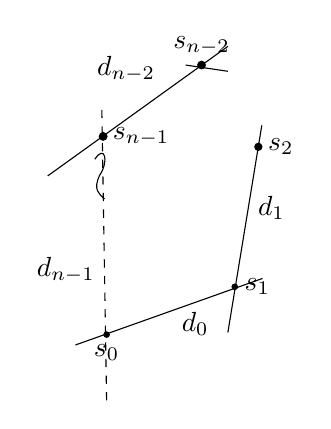
\begin{tikzpicture}[x=.88cm,y=.88cm]
\draw (-.45,-.15)--(2.25,.81) node[pos=.64,below] {$d_0$};
\draw (1.75,.03)--(2.24,3.02) node[pos=.60,right] {$d_1$};
\draw[dashed] (0,-.95)--(-.07,3.32) node[pos=.44,left] {$d_{n-1}$};
\draw (-.85,2.29)--(1.75,4.16) node[pos=.65,above left] {$d_{n-2}$};
\draw (1.14,3.89)--(1.75,3.80);
\draw (-.17,2.53) .. controls (-.03,2.75) and (.04,2.51) .. (-.10,2.30) .. controls (-.20,2.09) and (-.11,2.03) ..(-.03,1.96);
\fill (0,0) circle(1.2pt) node[below] {$s_0$};
\fill (1.85,.69) circle(1.2pt) node[right] {$s_1$};
\fill (2.19,2.71) circle(1.5pt) node[right] {$s_2$};
\fill (-.05,2.86) circle(1.6pt) node[right] {$s_{n-1}$};
\fill (1.37,3.89) circle(1.6pt) node[above] {$s_{n-2}$};
\end{tikzpicture}}

\[\resizebox{\ifdim\width>\linewidth\linewidth\else\width\fi}{!}{$\displaystyle
\begin{aligned}
 U_{\unsure{\underline{s}_0|\underline{s}0|\underline{S}_0}}={}&
 \Bigl\{\bigl((\unsure{p|P}_{\underline{s}})_{\underline{s}\in\underline S},
 (d_{\underline a})_{\underline a\in\underline A}\bigr)\in
 \unsure{\mathbb{P}\mathrm{ol}_n|\mathbb{P}\mathrm{P}_n}\Bigm|
 \begin{gathered}
 \inserted{d_{\underline a}}\\
 \deleted{p_{\underline{s}}\unsure{\notin|\in}(d_{\unsure{i-2|i-1|s-2}})_{\unsure{t}}}\\
 \deleted{\forall\,\unsure{t|b|s}\in S}
 \end{gathered}\Bigr\}
\end{aligned}
$}\]

\[
s_2\in d_0 \qquad s_0,d_0,s_1,d_1,\ldots s_{n-3},d_{n-3},s_{n-2}
\]

\figure{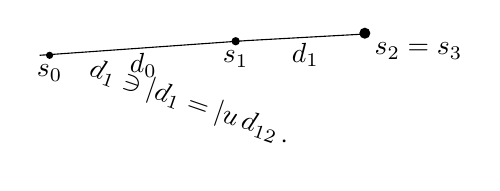
\begin{tikzpicture}[x=.85cm,y=.85cm]
\draw (-.15,0)--(2.95,.22)--(4.75,.32);
\fill (0,0) circle(1.3pt) node[below] {$s_0$};
\fill (2.78,.21) circle(1.5pt) node[below] {$s_1$};
\fill (4.71,.33) circle(2pt) node[below right] {$s_2=s_3$};
\node at (1.4,-.15) {$d_0$}; \node at (3.82,.00) {$d_1$};
\node[rotate=-19] at (2.10,-.72) {$\unsure{\shortparallel d_1\ni|\shortparallel d_1=|u\,d_{12}}\,.$};
\end{tikzpicture}\hspace{1cm}
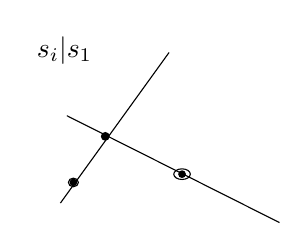
\begin{tikzpicture}[x=.75cm,y=.75cm]
\draw (-.76,-1.13)--(1.08,1.42); \draw (-.65,.35)--(2.95,-1.46);
\fill (0,0) circle(1.6pt);
\fill (-.54,-.78) circle(1.4pt); \draw (-.54,-.78) ellipse (.085 and .073);
\fill (1.30,-.64) circle(1.4pt); \draw (1.30,-.64) ellipse (.14 and .09);
\node at (-.69,1.45) {$\unsure{s_i|s_1}$};
\end{tikzpicture}}

\[\resizebox{\ifdim\width>\linewidth\linewidth\else\width\fi}{!}{$\displaystyle
\begin{aligned}
\underbrace{d_0=d_1\ \cdots\ =d_i}&\ne d_{i+1}\\[-2pt]
\rotatebox{-25}{$\Downarrow$} &\qquad\Downarrow\\[-4pt]
s_0,s_1,\ldots s_{i+2} &\qquad s_{i+2}
\end{aligned}
$}\]

\figure{\begin{tikzpicture}[x=.90cm,y=.90cm]
\draw (0,0)--(5.55,0)--(7.53,1.78) node[midway,below right] {$d_{i+1}$};
\fill (0,0) circle(1.2pt) node[below left] {$s_0$};
\fill (3.66,0) circle(1.2pt) node[below] {$s_i$};
\fill (5.55,0) circle(2.2pt) node[below right] {$s_{i+1}=s_{i+2}$};
\node at (1.9,-.65) {$d_0=\cdots=d_i$};
\end{tikzpicture}}

\figure{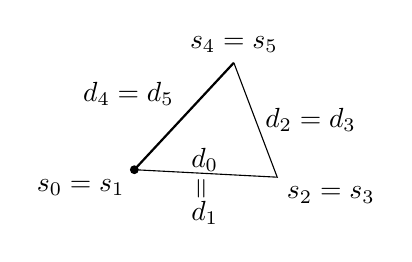
\begin{tikzpicture}[x=.95cm,y=.95cm]
\draw[thick] (0,0)--(1.33,1.43) node[midway,above left] {$d_4=d_5$};
\draw (1.33,1.43)--(1.91,-.10) node[midway,right] {$d_2=d_3$} --(0,0);
\fill (0,0) circle(1.6pt) node[below left] {$s_0=s_1$};
\node[above] at (1.33,1.43) {$s_4=s_5$};
\node[below right] at (1.91,-.10) {$s_2=s_3$};
\node at (.94,.13) {$d_0$};\node[rotate=90] at (.92,-.26) {$=$};\node at (.94,-.58) {$d_1$};
\end{tikzpicture}}
% archive sheet number: 3
\scanpage{4}

\[\resizebox{\ifdim\width>\linewidth\linewidth\else\width\fi}{!}{$\displaystyle
\begin{aligned}
 L_0(\lambda)\sigma&=0 & L_0(\lambda)&=L_1(\lambda) & \Sigma\\
 L_1(\lambda)\sigma&=0\\
 \deleted{\unsure{L_2(\lambda)\sigma=0|u_2(\lambda)\sigma=0}}&&L(\lambda)\sigma&=
\end{aligned}
$}\]
\[
 u\sigma=0\qquad
 \underbrace{L_0=L_1\ \cdots\ =L_{n-2}}_{u}\quad L_{n-1}
\]
\[
 \underbrace{(L_{n-2}-L_{n-1})}_{M_{n-1}}\deleted{\unsure{=|\sigma}}u_{n-1}=u_0\sigma
\]
\[\resizebox{\ifdim\width>\linewidth\linewidth\else\width\fi}{!}{$\displaystyle
\begin{aligned}
 M_1u_1&=(L_0-L_{1})u_1
 =\lambda_0u_{\unsure{-1|-4}}u_{12}\deleted{\unsure{+}}\unsure{-}\lambda_1u_1u_{02}
 +\lambda_2u_1u_2\unsure{\big\backslash|)}=\\
 M_2u_2&=(L_1-L_2)u_2
 =(\lambda_0u_{-1}u_{13}-\lambda_1u_1u_{03})+\lambda_3u_2u_3\quad\mathrm{mod}
\end{aligned}
$}\]
% archive sheet number: 10
\scanpage{5}
\mspage{\textcircled{21}}

\[\resizebox{\ifdim\width>\linewidth\linewidth\else\width\fi}{!}{$\displaystyle
\begin{aligned}
 \lambda_2\deleted{u_1}u_2&=-\lambda_0u_{-1}\deleted{u_1}+
 \lambda_1\deleted{u_1}(u_0+u_1)\\
 \underbrace{\lambda_n}_{\lambda_0}u_{n-1}\underbrace{u_n}_{u_0}
 &=-\lambda_0\underbrace{u_{-1}}_{u_{n-1}}
 \underbrace{u_{1n}}_{u_{0n}-u_0}+\lambda_1u_1u_{0n}
\end{aligned}
$}\]

\noindent\begin{tikzpicture}[x=1cm,y=1cm]\draw (0,0)..controls (3,-.04) and (6,.08)..(6.6,.02)..controls (7.2,.01) and (7.55,.45)..(7.64,1.05);\end{tikzpicture}\quad
\unsure{revenant|revenons|arrivant} aux $\lambda_{\ast}$

la dim de la variété des \unsure{$\lambda_{\ast}$|$\mu_{\ast}$} tels que --- est $n-2$ \quad $(\subset P^{n-1})$ \uline{sans} la condition $\sum u_i=0$ est $n-4$ \uline{avec} la condition $\sum u_i=0$ \unsure{qui est|précisemt|présumt} de codim $3$ dans $P^{n-1}$

\margin{\resizebox{\marginparwidth}{!}{$\left\{\begin{aligned}
 &(\underline{C_1,\ldots,C_{n-2}})\\
 &1+C_1+C_{\unsure{3|5}}\deleted{\unsure{\sum}}\cdots+C_{n-3}=0\\
 &1+C_2+C_4\cdots+C_{n-2}=0
 \end{aligned}\right.$}}

\noindent\rule{\linewidth}{.4pt}

\unsure{Calculs intra-marginaux|Calculs intra marginaux|Calcul intrinsèque}

\[\resizebox{\ifdim\width>\linewidth\linewidth\else\width\fi}{!}{$\displaystyle
\begin{aligned}
 &\lambda_0\\
 &\deleted{u\quad u_1,u_1}\\
 &\underline{u_0,u_1}\qquad\deleted{\unsure{\lambda_\ast}}\,u\qquad
 \boxed{u_0,u_1\,;\,u}\\
 &\deleted{=\lambda_2u_2\unsure{-}\lambda}
\end{aligned}
$}\]
\[\resizebox{\ifdim\width>\linewidth\linewidth\else\width\fi}{!}{$\displaystyle
\begin{aligned}
u_1\quad &\lambda_1u_0-\lambda_2u_2=u&&\Longrightarrow u_2\\
u_2\quad &\lambda_2u_1-\lambda_3u_3=u&&\Longrightarrow u_3
 \quad\big|\quad\text{en fonction de }u_0,u_1,u\\
&\text{---}\\
u_{n-2}\quad &\lambda_{n-2}u_{n-3}-\lambda_{n-1}u_{n-1}=u&&\Longrightarrow u_{n-1}\\
u_{n-1}\quad &\lambda_{n-1}u_{n-2}-\lambda_n u_n=u&&\Longrightarrow
 \underset{\substack{\shortparallel\\u_0}}{u_n}\quad
 \text{relation entre }u_0,u_1,u,\lambda_{\ast}\\
u_n\quad &\lambda_n u_{n-1}-\lambda_{n+1}u_{\unsure{n+1|n-1}}=u&&\Longrightarrow
 \underset{\substack{\shortparallel\\u_1}}{u_{n+1}}\quad
 \text{relation entre }u_0,u_1,u,\lambda_{\ast}
\end{aligned}
$}\]
% archive sheet number: 11
\scanpage{6}

\diagram{\begin{tikzcd}[ampersand replacement=\&,row sep=small,column sep=small]
 \&s_2\arrow[dl,"u_2"']\&\\
 s_3\arrow[dr,"u_3"']\&\&s_1\arrow[ul,"u_1"']\\
 \&s_0\arrow[ur,"u_0"']\&
\end{tikzcd}}

\[
 \mu_0+\mu_2=\mu_1+\mu_3\qquad \mu_3=\mu_0-\mu_1+\mu_2
\]
\[\resizebox{\ifdim\width>\linewidth\linewidth\else\width\fi}{!}{$\displaystyle
\begin{aligned}
 &\deleted{\unsure{\Sigma(\lambda)_4=(\sigma_i)\in V^2|\Sigma(V)_4=(\sigma_i)\in V^2}_4}\\
 &\mathbb M_4\longrightarrow P^2
 &u_0\wedge u_2&=u_0\wedge(u_0+u_{\unsure{2|1}})\\
 &&&=\deleted{\unsure{+}}-u_0\wedge(u_1+u_3)\\
 &&&=-\underbrace{u_0\wedge u_1}_{\mu_1}+\underbrace{u_3\wedge u_0}_{\mu_0}
\end{aligned}
$}\]
\[\resizebox{\ifdim\width>\linewidth\linewidth\else\width\fi}{!}{$\displaystyle
(u_0,u_1,u_2,u_3)\longrightarrow
 \bigl(\underbrace{u_3\wedge u_0}_{\mu_0},
       \underbrace{u_0\wedge u_1}_{\mu_1},
       \underbrace{u_1\wedge u_2}_{\mu_2}\bigr).
$}\]
\[\resizebox{\ifdim\width>\linewidth\linewidth\else\width\fi}{!}{$\displaystyle
\begin{aligned}
 &\deleted{u_0\wedge u_2}\\
 u_0\wedge u_2&=\mu_0-\mu_1\\
 u_1\wedge u_3&=\mu_{\unsure{1|0}}-\mu_2\\
 u_2\wedge u_0&=\mu_2-\mu_3=\mu_1-\mu_0=-u_0\wedge u_2\\
 u_3\wedge u_1&=\mu_3-\mu_0=\mu_2-\mu_1=-u_1\wedge u_3
\end{aligned}
$}\]

$\mathbb M_4\longrightarrow P^2_{\mathbb Z}$ \deleted{injectif} mono (car la connaissance des $\mu_0,\mu_1,\mu_2$ implique celle des \deleted{$\mu_3$}, \unsure{donc|tous} les $u_i\wedge u_j$ \ldots)

épi ?

$\mu_0,\mu_1,\mu_2,\mu_3$ \deleted{\unsure{soit}} donnés, \qquad $\mu_0+\mu_2=\mu_1+\mu_3$, $\mu_i$ pas tous nuls

\unsure{OPS} $\mu_1\ne 0$

On prend $u_0,u_1$ comme base \inserted{\text{de }V}, $u_0\wedge u_1$ base \inserted{e} de $\bigwedge^2 V$
\[
 u_2=\alpha u_0+\beta u_1,\qquad u_3=-(u_0+u_1+u_2)
\]
\[\resizebox{\ifdim\width>\linewidth\linewidth\else\width\fi}{!}{$\displaystyle
\begin{aligned}
u_0\wedge u_1&=1.e & \mu'_1&=1\\
u_1\wedge u_2&=-\alpha e & \mu'_2&=-\alpha\\
u_2\wedge u_3&=(\deleted{\unsure{\alpha}}\beta-\deleted{\unsure{\beta}}\alpha)e
 & \underline{\mu'_3}&\underline{=\deleted{\unsure{\alpha}}\beta-\deleted{\unsure{\beta}}\alpha}\\
u_3\wedge u_0&=(1+\beta)e & \mu'_0&=1+\beta
\end{aligned}
\qquad
\begin{aligned}
u_2\wedge u_3&=-u_2\wedge u_0\unsure{-|+}u_2\wedge u_1\\
&=\beta\underbrace{u_0\wedge u_1}_{e}\deleted{\unsure{+}}-\alpha e\\
u_3\wedge u_0&=-u_1\wedge u_0-u_2\wedge u_0\\
&=\deleted{\unsure{1|V}}e+\beta e
\end{aligned}
$}\]
\[
 \alpha=-\frac{\mu_2}{\mu_1}\qquad
 \beta-\alpha=\frac{\mu_3}{\mu_1}\qquad \text{i.e.}\quad
 \beta=\frac{\mu_3}{\mu_1}+\alpha=\frac{\mu_3-\mu_2}{\mu_1}.
\]
\[\resizebox{\ifdim\width>\linewidth\linewidth\else\width\fi}{!}{$\displaystyle
\begin{aligned}
 u_2&=-\frac{\mu_2}{\mu_1}u_0+\frac{\mu_3-\mu_2}{\mu_1}u_1\\
 u_3&=\left(\frac{\mu_2}{\mu_1}-1\right)u_0+
 \underbrace{\frac{\mu_2-\mu_3-\mu_1}{\mu_1}}_{-\mu_0}u_1
\end{aligned}
\qquad
\begin{aligned}
 &\mathbb M_4\simeq P^2_{\mathbb Z}\\
 &u_2=0\Longleftrightarrow
 \left\{\begin{gathered}\deleted{\mu_1\ne0}\\ \boxed{\mu_2=0,\mu_3=0}\end{gathered}\right.\\
 &\hspace{2cm}\mu_0=\mu_1
\end{aligned}
$}\]

Les quadrilatères \unsure{épinglés}, \unsure{i.e.|ceux} avec un côté nul, correspondent aux quatre pts \inserted{a_i\ (i=0,1,\unsure{2|3},3)} de $P^2_{\mathbb Z}$ $(\deleted{\unsure{P^3}}\mu_0+\mu_2=\mu_1+\mu_3)\subset P^{\unsure{3|2}}$ $(\mu_0,\mu_1,\mu_2,\mu_3)$ correspondant à deux coordonnées \unsure{consec.|conséc.} $\mu_i$ nulles (les deux autres égales) \unsure{Il n'y a|Il n'y en a} pas $3$ dans \unsure{$a_i$|ces|ce} qui
% archive sheet number: 12
\scanpage{7}

soient alignés (p.ex les vecteurs .
\[
 (0,0,1,1)\quad(1,0,0,1)\quad(1,1,0,0)
\]
ne sont pas coplanaires \deleted{\unsure{les}} i.e la matrice
\[
 \begin{pmatrix}0&0&1&1\\1&0&0&1\\1&1&0&0\end{pmatrix}
 \quad\text{de rang }3\ \ldots)
\]

Donc ils forment une base projective de $P^2$, donc, \deleted{\unsure{$M_4\simeq$}} si $\Pi=(S,A)$ est un quadrilatère combinatoire, $\mathbb M(\Pi)$ s'identifie à l'enveloppe projective de $A$.

\figure{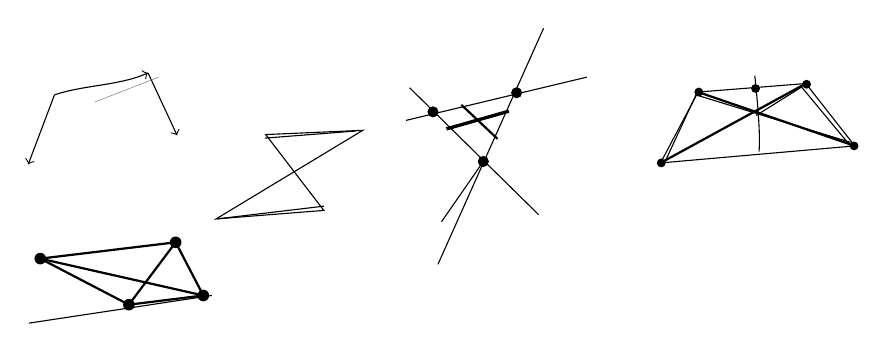
\begin{tikzpicture}[x=.009cm,y=-.009cm]
\draw[->] (149,990)--(112,1088);
\draw[->] (149,990)..controls(190,976)and(241,977)..(281,959);
\draw[->] (281,959)--(322,1047);
\draw[very thin,gray] (206,1000)--(296,965);
\draw (377,1165)--(584,1040)--(447,1046)--(529,1153)--cycle;
\draw[thin] (378,1165)--(529,1147) (446,1051)--(574,1041);
\draw (645,1026)--(900,965) (650,980)--(832,1159) (690,1229)--(839,896);
\draw (695,1169)--(754,1084); \draw[very thick] (702,1038)--(790,1013);
\draw[thick] (723,1004)--(774,1052);
\foreach \x/\y in {683/1014,801/987,754/1084}{\fill (\x,\y) circle(2pt);}
\draw (1004,1086)--(1057,986)--(1209,974)--(1278,1062)--cycle;
\draw[thick] (1004,1086)--(1209,974) (1057,986)--(1278,1062);
\draw (1137,963)..controls(1140,994)and(1145,1039)..(1143,1070);
\draw[thin] (1010,1085)--(1054,990)--(1272,1057) (1139,1019)--(1203,979)--(1271,1061);
\foreach \x/\y in {1005/1086,1058/986,1210/975,1277/1062,1138/981}{\fill (\x,\y) circle(1.6pt);}
\draw (113,1312)--(371,1273); \draw[thick] (129,1221)--(320,1198)--(359,1273)--(254,1286)--cycle;
\draw[thick] (129,1221)--(359,1273) (254,1286)--(320,1198);
\foreach \x/\y in {129/1221,320/1198,359/1273,254/1286}{\fill (\x,\y) circle(2.1pt);}
\end{tikzpicture}}
% archive sheet number: 13
\scanpage{9}

\[\resizebox{\ifdim\width>\linewidth\linewidth\else\width\fi}{!}{$\displaystyle
\begin{aligned}
 &\deleted{\mathcal F_\nu\subset\widetilde\Omega^\nu}\\
 &\mathcal F_\nu\subset
 \underset{\substack{\shortparallel\\
 \operatorname{Im}\bigl((C\times\Omega^\nu)\unsure{\longrightarrow|\text{---}}\widetilde\Omega^\nu\bigr)}}{T_\nu}
 \subset\widetilde\Omega^\nu\\
 &\mathcal F_i\subset T_i\subset\widetilde\Omega^i\qquad 1\leq i\leq\nu\\
 &\operatorname{pr}_{\deleted{\nu}i-1,\deleted{\nu}i}
  (\mathcal F_{\deleted{\nu}i})\subset\mathcal F_{i-1}\qquad 2\leq i\leq\nu\\
 &\mathcal F_{\deleted{\nu}i}=
 ((\widetilde\omega_1,\ldots\widetilde\omega_i)\mid
  (\widetilde\omega_1,\ldots\widetilde\omega_{i-1})\in\mathcal F_{i-1},\ \omega_i\\
 &\hspace{5.4cm}\widetilde\Omega^{\deleted{\nu}i-1}\times\Omega\\
 &\mathcal F_i=T_i\cap(\widetilde\Omega^{i-1}\times\widetilde\Omega\mid\mathcal F_{i-1}
 \qquad T_{i-1}\times\Omega
\end{aligned}
$}\]
\[\resizebox{\ifdim\width>\linewidth\linewidth\else\width\fi}{!}{$\displaystyle
\begin{aligned}
f_1&\subset\Omega\\
f_2&\subset\widetilde\Omega\times\Omega\\
&\cdots\\
f_i&\subset\widetilde\Omega^{i-1}\times\Omega\\
&\subset T_{i-1}\times\Omega.\\
&\cdots\\
f_\nu&\subset\widetilde\Omega^{\nu-1}\times\Omega
\end{aligned}
$}\]
\diagram{\begin{tikzcd}[ampersand replacement=\&,row sep=small,column sep=small]
 \widetilde\Omega^{i-1}\times\Omega \& {\ni f_i}\\
 \unsure{f_{\deleted{\mathrm{pr}}}|{\uparrow}\deleted{\mathrm{pr}}} \&\\
 \widetilde\Omega^i \& \mathcal F_i\\
 \widetilde\Omega^{\deleted{\nu}i}\times\Omega\arrow[u,"\mathrm{pr}_1"] \& {\supset f_{i+1}}
\end{tikzcd}}

\[\resizebox{\ifdim\width>\linewidth\linewidth\else\width\fi}{!}{$\displaystyle
 \deleted{\mathcal F_i}\quad
 \left\{\begin{aligned}
 &\deleted{f_i\subset T_{i-1}\times\Omega}\\
 &\underset{\substack{\cap\\\widetilde\Omega^i}}{\mathcal F_i}
 =\bigl\{(\widetilde\omega_1(x)\ldots\widetilde\omega_{i-1}(x),\omega_i(x))\bigm|
 \begin{gathered}x\in C\\\omega_1\ldots\omega_i\in\Omega^i\end{gathered}
 \inserted{\text{t.q.}}\ 
 (\omega_1(x),\ldots\omega_{i-1}(x),\unsure{\omega_i|\omega_i(x)})\in f_i\bigr\}
 \end{aligned}\right.
$}\]
\[\resizebox{\ifdim\width>\linewidth\linewidth\else\width\fi}{!}{$\displaystyle
\begin{aligned}
 &f_i\subset T_{i-1}\times\Omega\subset\widetilde\Omega^{i-1}\times\Omega\\
 \text{\unsure{surj|sur}}\ {\uparrow}\quad &\hspace{6cm}\nwarrow\\
 \mathcal F_i=\widetilde f_i&\unsure{\in|\subset} T_i\quad\subset
 \widetilde\Omega^{i-1}\times\widetilde\Omega=\widetilde\Omega^i\\
 &\shortparallel\quad T_i\cap(\deleted{\unsure{f_i\times}}\widetilde\Omega^i\mid f_i)
\end{aligned}
$}\]

% margin note written sideways
\margin{\resizebox{\marginparwidth}{!}{\(\begin{array}{ll}
\bullet\,\text{\unsure{Mum Br.|Mum Dr.|Mme Dr.}}&\text{\deleted{\unsure{Julia}}}\\
\bullet\,\text{\unsure{Justine|Jyptine}}&\text{\unsure{Mireille}}\\
\text{\deleted{\unsure{Sina|Sima}}}&\text{\uline{\unsure{Julia}}}\\
\text{\unsure{Nava|Nara}}&\text{\deleted{\unsure{Christophe|Christoph}}}\\
\bullet\,\text{\unsure{Sokina|Sokine}}&\text{\unsure{Sylvie}}\\
 &\text{\deleted{\unsure{Anne}}}\\
 &\text{\unsure{Sindy|Sinty}}
\end{array}\)}}
% archive sheet number: 15
\scanpage{10}

\[\resizebox{\ifdim\width>\linewidth\linewidth\else\width\fi}{!}{$\displaystyle
 \boxed{\mathcal F_1\subset\Omega_{\deleted{\unsure{1}}}}
 \quad\deleted{\unsure{\varnothing}}\quad \text{i.e.}\quad
 \mathcal F_1\in{\unsure{\mathscr P|\wp|\mathfrak P}}^{\ast}(\Omega)
$}\]
\[
 \widetilde{\mathcal F}_1=(\widetilde\Omega\mid\mathcal F_1)\cap T_1
 \quad\subset\widetilde\Omega=\widetilde\Omega_1
\]
\[
 \boxed{f_2:\widetilde{\mathcal F}_1\longrightarrow\mathscr P^\ast(\Omega)}
 \qquad\widetilde\Omega\times\Omega
\]

$\deleted{\unsure{\widetilde{\mathcal F}_1}}\
(\widetilde\omega_1,\omega_2)\in\widetilde\Omega\times\Omega$ comp. avec $(\mathcal F_1,\mathcal F_2)$ si
\[\resizebox{\ifdim\width>\linewidth\linewidth\else\width\fi}{!}{$\displaystyle
\begin{aligned}
 &\text{a)}\quad\widetilde\omega_1\in\widetilde{\mathcal F}_1
 \quad\text{i.e.}\quad\omega_1\in\mathcal F_1\text{ et }\widetilde\omega_1\in T_1\\
 &\deleted{\text{b)}\quad\widetilde\omega_1\in T_1}\\
 &\text{b)}\quad\omega_2\in f_2(\widetilde\omega_1)
\end{aligned}
$}\]
\[\resizebox{\ifdim\width>\linewidth\linewidth\else\width\fi}{!}{$\displaystyle
\begin{aligned}
 \widetilde{\mathcal F}_2\subset\widetilde\Omega_2
 =\widetilde\Omega\times\widetilde\Omega\ \unsure{\ni|=}\ 
 \bigl\{(\widetilde\omega_1,\omega_2)\bigm|&
 \omega_1\in\mathcal F_1,\,
 (\widetilde\omega_1\times\widetilde\omega_2)\in T_2,\\
 &\widetilde\omega_2\in f_2(\widetilde\omega_1)\bigr\}
\end{aligned}
$}\]
\[
 f_3:\widetilde{\mathcal F}_2\longrightarrow\mathscr P(\Omega)
\]
\[\resizebox{\ifdim\width>\linewidth\linewidth\else\width\fi}{!}{$\displaystyle
\begin{aligned}
 &\cdots\\
 &f_\nu:\underset{\substack{\cap\\\widetilde\Omega^{\nu-1}}}{\widetilde{\mathcal F}_{\nu-1}}
 \longrightarrow\mathscr P(\Omega)\qquad\text{\unsure{d'où|déf|donc}}\\
 &\widetilde{\mathcal F}_\nu\subset\widetilde\Omega^\nu\quad
 \text{(en fait, }\widetilde{\mathcal F}_\nu\subset T_\nu)
\end{aligned}
$}\]

$(\mathcal F_1,\ldots,\mathcal F_\nu)$ est appelé \unsure{une|un} \deleted{\unsure{multiplicité|multiplet} de} \inserted{\text{crible de \uuline{longueur $\nu$}}}

\uline{NB} \unsure{certains|Certains} $\widetilde{\mathcal F}_i$ peuvent \unsure{être|etre} $\varnothing$

\[\resizebox{\ifdim\width>\linewidth\linewidth\else\width\fi}{!}{$\displaystyle
\begin{aligned}
 \mathcal F_1&=f_1\subset\Omega
 &\widetilde\Omega\times\widetilde\Omega\ \cdots\ \times\widetilde\Omega\\
 \mathcal F_2&\subset\widetilde\Omega\times\Omega&\mathcal F\\
 \mathcal F_3&\subset\widetilde\Omega\times\widetilde\Omega\times\Omega\\
 &\cdots\\
 \mathcal F_\nu&\subset
 \underbrace{\widetilde\Omega\times\widetilde\Omega\ \cdots\ \widetilde\Omega}_{\nu-1}\times\Omega
\end{aligned}
$}\]
% archive sheet number: 16
\scanpage{11}

$C$ ``configurations''

$\Omega$ ``opérations'' (virtuelles)

\[\resizebox{\ifdim\width>\linewidth\linewidth\else\width\fi}{!}{$\displaystyle
 \omega\in\Omega\qquad
 \omega\longmapsto\bigl(f_\omega:C\longrightarrow
 \underset{\substack{\shortparallel\\\text{\scriptsize ``ens. des résultats \inserted{\text{virtuels}} des l'opération }\omega}}{V_\omega}\bigr)
$}\]
\margin{On pose $f_\omega(x)=\omega(x)$}

$\widetilde\Omega$ ``opérations effectuées'' :
\[
 \widetilde\Omega=\coprod_{\omega\in\Omega}V_\omega
 \xrightarrow{\pi}\Omega
\]
\[\resizebox{\ifdim\width>\linewidth\linewidth\else\width\fi}{!}{$\displaystyle
\left\{\begin{aligned}
 C(\omega,x)&=f_\omega^{-1}(\{\deleted{\unsure{f}}f_\omega(x)\})&
 \text{ombre de \inserted{\text{la conf.}} }x\in C\text{ pour l'op }\omega.\\
 &=C(\omega(x))\\
 &\text{de même on définit}\\
 C(\omega_1,\ldots\omega_\nu\,;x)&=\bigcap_{1\leq i\leq\nu}C(\omega_i\,;x)&
 \text{ombre de }x\in C\text{ pour}\\
 &&\text{la suite d'op. }\omega_1\ldots\omega_\nu
\end{aligned}\right.
$}\]

\[\resizebox{\ifdim\width>\linewidth\linewidth\else\width\fi}{!}{$\displaystyle
\begin{aligned}
 \widetilde\Omega&\xrightarrow{\widetilde\omega\mapsto C(\widetilde\omega)}
 \unsure{\mathscr P|\wp|\mathfrak P}(C)\\
 \widetilde\omega=(\omega,v)&\longmapsto f_\omega^{-1}(\{v\})
\end{aligned}
$}\]
\margin{\uline{NB} \unsure{OPS} pour la suite que les $f_\omega$ sont surj}

\[
 \widetilde\omega\longmapsto C(\widetilde\omega)
 \qquad\text{ensemble résiduel pour l'op. eff. }\widetilde\omega
\]
\[\resizebox{\ifdim\width>\linewidth\linewidth\else\width\fi}{!}{$\displaystyle
\begin{aligned}
 \widetilde\Omega^\nu&\unsure{\longrightarrow|\text{---}}\mathscr P(C)\\
 (\widetilde\omega_1,\ldots,\widetilde\omega_\nu)&\longmapsto
 C(\widetilde\omega_1,\ldots,\widetilde\omega_\nu)
 =\bigcap_{1\leq i\leq\nu}C(\widetilde\omega_i)
\end{aligned}
$}\]

ensemble résiduel pour la suite d'opérations \unsure{effectives|effectuées} $\widetilde\omega_1\ldots\widetilde\omega_\nu$.

\[\resizebox{\ifdim\width>\linewidth\linewidth\else\width\fi}{!}{$\displaystyle
\begin{aligned}
 \Omega^\nu&\ \tikz[baseline=-.2ex,x=1cm,y=1cm]{\draw[->] (0,.88)..controls(-.09,.88) and (-.10,.44)..(-.09,.30)..controls(-.09,.23) and (.04,.18)..(.48,0);}\ \text{\uline{tests} virtuels de longueur }\nu\\
 T_\nu\subset\widetilde\Omega^\nu&\quad\text{--- effectués de longueur }\nu
\end{aligned}
$}\]
\[\resizebox{\ifdim\width>\linewidth\linewidth\else\width\fi}{!}{$\displaystyle
\begin{aligned}
 C\times\Omega&\longrightarrow\widetilde\Omega\quad\deleted{\unsure{\longrightarrow|\Longleftrightarrow|\Longrightarrow}}&
 C&\longrightarrow\Gamma(\widetilde\Omega/\Omega)\\
 (x,\omega)&\longmapsto\omega(x)&
 C\times\Omega^\nu&\longrightarrow\widetilde\Omega^\nu
\end{aligned}
$}\]
\[\resizebox{\ifdim\width>\linewidth\linewidth\else\width\fi}{!}{$\displaystyle
\begin{aligned}
 C&\longrightarrow\deleted{\unsure{\Omega}}\Gamma(\widetilde\Omega^\nu/\Omega^\nu)\\
 x&\longmapsto\bigl((\omega_1,\ldots,\omega_\nu)\longmapsto
 (\omega_1(x),\ldots,\omega_\nu(x))\bigr)
\end{aligned}
$}\]

l'image de $C\times\Omega^\nu$ est appellée ens des tests \deleted{\unsure{effectués}} \inserted{\text{\unsure{effectifs|effectués}}} de lg. $\nu$. Soit $T_\nu$ l'ens de ceux-ci.
% archive sheet number: 17
\scanpage{13}

\figure{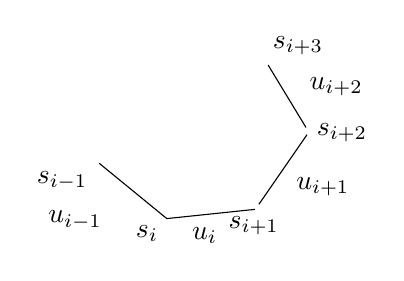
\begin{tikzpicture}[x=.013cm,y=-.013cm]
\draw (102,151)--(168,205)--(254,196);
\draw (258,191)--(305,123); \draw (304,116)--(267,55);
\node[left] at (100,168) {$\unsure{s}_{i-1}$};
\node[below left] at (114,188) {$u_{i-1}$};
\node[below left] at (169,202) {$s_i$};\node[below] at (205,204) {$u_i$};
\node[below] at (253,193) {$s_{i+1}$};\node[right] at (285,174) {$u_{i+1}$};
\node[right] at (305,121) {$s_{i+2}$};\node[right] at (298,76) {$u_{i+2}$};
\node[above right] at (262,55) {$s_{i+3}$};
\end{tikzpicture}}

\[\resizebox{\ifdim\width>\linewidth\linewidth\else\width\fi}{!}{$\displaystyle
\begin{aligned}
 \text{hyp \unsure{de donn.|donn.|données}}\quad&
 \left\{\begin{aligned}u&=\lambda_i u_{i-1}-\lambda_{i+1}u_{i+1}
 \qquad i=0,1,\ldots,n-1\\ \sum u_i&=0\end{aligned}\right.\\
 \text{(\unsure{def|déf})}\quad&
 \left\{\begin{aligned}u_{i-1}\wedge u_i&=\mu_i\\u\wedge u_i&=\alpha_i\end{aligned}\right.
 \quad\deleted{\unsure{\big\}\ (\mathrm{def})}}
\end{aligned}
$}\]
\[
 \deleted{u\ne0\quad
 \left.\begin{gathered}u_i\ne0\\\lambda_i\ne0\end{gathered}\right\}\forall i
 \quad\Longrightarrow(\unsure{\alpha|u_i})_i\ne}
\]
\[\resizebox{\ifdim\width>\linewidth\linewidth\else\width\fi}{!}{$\displaystyle
 \underbrace{\left.\begin{aligned}(\mu_i)_i&\ne0\ -\\
 \text{et }\ u&\ne0\end{aligned}\right\}\Longleftrightarrow(\alpha_i)_i\ne0}_{\text{hyp}}
 \qquad\unsure{\text{et}}\quad
 \underbrace{u_i\ne0,\ \lambda_i\ne0\quad\forall i}_{\text{hyp.}}
$}\]
\[\resizebox{\ifdim\width>\linewidth\linewidth\else\width\fi}{!}{$\displaystyle
 \left\{\begin{aligned}
 \lambda_i\mu_i+\lambda_{i+1}\mu_{i+1}&=\alpha_i\\
 \lambda_i\alpha_{i-1}-\lambda_{i+1}\alpha_{i+1}&=0\\
 \sum\alpha_i&=0\qquad 2\sum\lambda_i\mu_i=0
 \end{aligned}\right.
 \qquad
 \begin{aligned}(\lambda_i,\alpha_i)_i&\ne0\\
 &P(k^n\times L^n)\end{aligned}
$}\]
\deleted{\unsure{($\lambda_i$) connu quand on connaît}}

\[\resizebox{\ifdim\width>\linewidth\linewidth\else\width\fi}{!}{$\displaystyle
\begin{aligned}
 u_0,u_1,u,(\lambda_i)&\Longrightarrow u_i\quad\forall\ \deleted{\unsure{\in}}i\\
 \alpha_0,\alpha_1,(\lambda_{\unsure{0|i}})&
 \underset{\text{si }\mu_1\ne0}{\Longrightarrow}(u_i)\ \text{mod Gp Aff}
\end{aligned}
$}\]
\[\resizebox{\ifdim\width>\linewidth\linewidth\else\width\fi}{!}{$\displaystyle
\begin{aligned}
 &\deleted{\unsure{(\alpha_i),(\lambda_i)}}\\
 u&=\frac{\alpha_1}{\mu_1}u_0-\frac{\alpha_0}{\mu_1}u_1
 =\left(\lambda_1+\lambda_2\frac{\mu_2}{\mu_1}\right)u_0-
 \left(\lambda_0\frac{\mu_0}{\mu_1}+\lambda_1\right)u_1\\
 &(\lambda_i,\deleted{\unsure{\alpha_i}}\mu_i)_i\quad\text{mod }k^\ast\quad .
\end{aligned}
$}\]

$CI_n^\ast={}$ $n$-polygônes critiques (mod Aff) \deleted{\unsure{de qui}} qui ne sont \unsure{en !|pas !} \deleted{\unsure{$\lambda_i\ne0\ \forall i$}} \deleted{\unsure{multi}}triangulaires

\[\resizebox{\ifdim\width>\linewidth\linewidth\else\width\fi}{!}{$\displaystyle
 \begin{aligned} &\big\downarrow\\&P^{n-1}\times P^{n-1}\\
 &(\lambda_i)\qquad(\mu_{\unsure{j|i}})\end{aligned}
 \qquad
 \begin{aligned}
 \deleted{\unsure{\lambda_2}}u_2&=-\deleted{\unsure{\lambda_2}}\frac{\mu_2}{\mu_1}u_0+
 \frac{1}{\lambda_2}\left(\lambda_0\frac{\mu_0}{\mu_1}+\lambda_1\right)u_1\\
 &\cdots\\
 u_{n-1}&=A_{n-1}\bigl((\lambda)(\mu)\bigr)u_0+B_{n-1}(\ ,\ )u_1
 \end{aligned}
$}\]
% archive sheet number: 19
\scanpage{15}
\mspage{\textcircled{\unsure{1|4}}}

\figure{\begin{tikzpicture}[x=.012cm,y=-.012cm]
\draw (369,218)--(584,116)--(755,209);
\node[above] at (442,140) {$u_{i-1}$};\node[above] at (582,112) {$s_i$};
\node[above] at (674,150) {$u_i$};\node[above right] at (747,206) {$s_{i+1}$};
\end{tikzpicture}}
\[
\begin{aligned}
 f_i&=x_{i-1}y_i-y_{i-1}x_i\\
 df_i&=y_i\,dx_{i-1}-x_i\,dy_{i-1}\unsure{-|+}
 (y_{i-1}\,dx_i-x_{i-1}\,dy_i)
\end{aligned}
\]
\[\resizebox{\ifdim\width>\linewidth\linewidth\else\width\fi}{!}{$\displaystyle
\begin{aligned}
 \sum\lambda_i\,df_i&=\sum_i(-\lambda_i y_{i-1}+\lambda_{i+1}y_{i+1})\,dx_i
 +\sum_i(\lambda_i x_{i-1}-\lambda_{i+1}x_{i+1})\,dy_i\\
 &\deleted{=\mu\sum dx_i+\nu\sum dy_i}\\
 &=\mu\sum dx_i+\nu\sum dy_{\unsure{i}}
\end{aligned}
$}\]
\[\resizebox{\ifdim\width>\linewidth\linewidth\else\width\fi}{!}{$\displaystyle
 \left.\begin{aligned}
 -\mu&=+\lambda_i y_{i-1}-\lambda_{i+1}y_{i+1}\\
 \nu&=+\lambda_i x_{i-1}-\lambda_{\unsure{i-1|i+1}}x_{\unsure{i+1|i-1}}
 \end{aligned}\right\}
 \quad 0\leq i\leq n-1
$}\]

\uuline{NB} \uline{OPS} $x_i,y_i$ tous $\ne0$ (par \unsure{chgt} de coord)

\[\resizebox{\ifdim\width>\linewidth\linewidth\else\width\fi}{!}{$\displaystyle
 \lambda_0,\lambda_1\mid
 \overset{\underline{i=1}}{\lambda_2}\ \cdots\
 \overset{\underline{i=n-2}}{\lambda_{n-1}}
 \qquad\overset{\underline{i=n-1}}{\text{\textcircled{$\lambda_n$}}}
 \quad\text{\unsure{relation|relations}}
$}\]

\[\resizebox{\ifdim\width>\linewidth\linewidth\else\width\fi}{!}{$\displaystyle
\begin{aligned}
 +\lambda_0 y_{n-1}\unsure{-|+}\lambda_1y_1
 &=+\lambda_1y_0-\lambda_2y_2=+\lambda_2y_1-\lambda_3y_3
 =\cdots=\lambda_{n-2}y_{n-3}-\lambda_{n-1}y_{n-1}\\
 &=\lambda_3y_2-\lambda_4y_4\qquad
 =\lambda_{n-1}y_{n-2}-\underbrace{\lambda_n}_{\shortparallel\,\lambda_0}
 \underbrace{y_n}_{\shortparallel\,y_0}\\
 &=\lambda_4y_3-\lambda_5y_5
\end{aligned}
$}\]

\[\resizebox{\ifdim\width>\linewidth\linewidth\else\width\fi}{!}{$\displaystyle
\begin{aligned}
 (y_2)\lambda_2&=\lambda_1(y_0+y_1)-\lambda_0y_{n-1}
 =\lambda_0(-y_{n-1})+\lambda_1(y_0+y_1)\\
 (y_2y_3)\lambda_3&=\underbrace{(y_2\lambda_{\unsure{1|2}})}y_1
 -y_2(\lambda_0y_{n-1}-\lambda_1y_1)\\
 &=\lambda_0(\deleted{\unsure{y_0}}\inserted{-}y_{n-1}(y_1+y_2))
 +\lambda_1y_1[\,y_0+y_1+y_2\,]\\
 (\underset{\longrightarrow}{\deleted{y_2}y_3}y_4)\lambda_4&=(y_2y_3\lambda_3)\underset{\smile}{\deleted{y_2}}
 -y_2y_3(\lambda_0y_{n-1}-\lambda_1y_1)\\
 &=\lambda_0(-y_2y_{n-1}(y_1+y_2+y_3))
 +\lambda_1y_1y_2(y_0+y_1+y_2+y_3)\\
 (y_2y_3y_4y_5)\lambda_5&=(\underbrace{y_2y_3y_4\lambda_4})y_3
 -y_2y_3y_4(\lambda_0y_{n-1}-\lambda_1y_1)
\end{aligned}
$}\]
% archive sheet number: 21
\scanpage{16}
\mspage{\textcircled{2}}

\[
 =\lambda_0\bigl(-y_{n-1}y_2y_3(y_1+y_2+y_3+y_4)\bigr)
 +\lambda_1y_1y_2y_3(y_0+y_1+y_2+y_3+y_4)
\]
\[
 \deleted{\unsure{y_2}y_3\cdots y_i\lambda_i
 =\lambda_0(-y_{n-1}y_2y_3\cdots y_{i-2}(y_1+\cdots+y_{i-1})
 +\lambda_1\unsure{y}}
\]
\[\resizebox{\ifdim\width>\linewidth\linewidth\else\width\fi}{!}{$\displaystyle
 \boxed{\begin{aligned}
 (y_{i-1}y_{\unsure{\nu|i}})\lambda_i
 &=(-\lambda_0\deleted{\unsure{y}}y_{-1})(y_1+\cdots+y_{i-1})\bigr]
 +(\lambda_1y_1)(y_0+\cdots+y_{i-1})\\
 (x_{i-1}x_i)\lambda_i&=(-\lambda_0x_{-1})(x_1+\cdots+x_{i-1})
 +(\lambda_1x_1)(x_0+\cdots+x_{i-1})
 \end{aligned}}
$}\]
\[
 i=2,\ldots n-1\ //\ n\qquad
 \boxed{\lambda_i u_{i-1}u_i=-\lambda_0u_{-1}u_{1i}+\lambda_1u_1u_{0i}}
\]
\[
 \text{où.}\quad u_{\alpha\beta}=u_\alpha+u_{\alpha+1}+\cdots+u_{\beta\unsure{+1|-1}}
 =s_\beta-s_\alpha
\]
\[\resizebox{\ifdim\width>\linewidth\linewidth\else\width\fi}{!}{$\displaystyle
 \boxed{\boxed{\begin{aligned}
 &\lambda_0\bigl[-x_{i-1}x_iy_{-1}(y_1+\cdots+y_{i-1})
 +y_{i-1}y_ix_{-1}(x_1+\cdots+x_{i-1})\bigr]\\
 &\quad+\lambda_1\bigl[x_{i-1}x_iy_1(y_0+\cdots+y_{i-1})
 -y_{i-1}y_ix_1(x_0+\cdots+x_{i-1})\bigr]=0
 \end{aligned}}}
 \quad\text{\tikz[baseline=(n.base)]\node[draw,rounded corners=8pt](n){$i=2,\ldots,n-1$};}
$}\]
\[\resizebox{\ifdim\width>\linewidth\linewidth\else\width\fi}{!}{$\displaystyle
 (\underbrace{y_{n-1}}_{y_{-1}}\underbrace{y_n}_{y_0})
 \underbrace{\lambda_n}_{\substack{\shortparallel\\\lambda_0}}
 =(-\lambda_0y_{-1})\underbrace{(y_1+\cdots+y_{n-1})}_{-y_0}
 +(\lambda_1y_1)\underbrace{(y_0+\cdots+y_{n-1})}_{\substack{\shortparallel\\0}}
$}\]
\[
 \lambda_0(y_{n-1}y_0)=\lambda_0 y_0y_{-1}\qquad\text{OK}
\]

\noindent\rule{\linewidth}{.4pt}

\uline{\unsure{triangles|triangle}}
\[\resizebox{\ifdim\width>\linewidth\linewidth\else\width\fi}{!}{$\displaystyle
\begin{aligned}
 &\lambda_0\bigl(-x_1x_2y_{-1}\underbrace{\deleted{(y_1+y_2)}}_{-y_0}
 +y_1y_2x_{-1}\underbrace{\deleted{(x_1+x_2)}}_{-x_0}\bigr)\\
 &\quad+x_1\underline{x_2y_2}(y_0\deleted{\unsure{+y_1}})
 \unsure{-|+}y_1\underline{y_2x_2}(\deleted{x_0+x_{\unsure{2|1}}})\\
 &\deleted{x_2y_2x_1y_1\Bigl[-\frac{y_1+y_2}{y_1}+\frac{x_1+x_2}{x_1}}\\
 &x_2y_2(x_1y_0-y_1x_0)
\end{aligned}
\qquad
\begin{aligned}
 &u\quad v\quad w=-(u+v)\\
 &u\wedge v\quad v\wedge w\quad w\wedge u\\
 &u\wedge v,\ -v\wedge u=u\wedge\unsure{v|w}\quad -v\wedge u=u\wedge v
\end{aligned}
$}\]
% archive sheet number: 22
\scanpage{17}
\mspage{\textcircled{3}}

\unsure{quadrilatère|quadrilatere}

\[\resizebox{\ifdim\width>\linewidth\linewidth\else\width\fi}{!}{$\displaystyle
\begin{aligned}
 &-x_1x_2y_{\deleted{\unsure{3}}1}y_{\deleted{\unsure{1}}3}
 +y_1y_2x_1x_3\\
 &\tikz[baseline=(n.base)]\node[draw,rounded corners=12pt](n){$=-x_{1}y_1(x_2y_3-y_2x_3)$};
\end{aligned}
$}\]

\noindent\rule{.6\linewidth}{.4pt}

\[\resizebox{\ifdim\width>\linewidth\linewidth\else\width\fi}{!}{$\displaystyle
\begin{aligned}
 &x_1x_2y_1\underbrace{(y_0+y_1)}_{-y_2-y_3}
 -y_1y_2x_1\underbrace{(x_0+x_1)}_{-x_2-x_3}=\\
 &=-x_1x_2y_1(y_2+y_3)+y_1y_2x_1(x_2+x_3)\\
 &=-\underline{x_1x_2y_1}y_3+\underline{y_1y_2x_1}x_3
 \quad\tikz[baseline=(n.base)]\node[draw,rounded corners=12pt](n){$=-x_1y_1(x_2y_3-y_2x_3)$};
\end{aligned}
$}\]
\[
 \boxed{\lambda_0+\lambda_1=0}
\]
\tikz[baseline=(c.base)]\node[draw,rounded corners=7pt,inner sep=2pt](c){si};\uline{ $s_3$ non aplati}
\figure{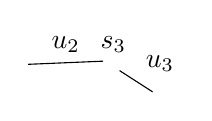
\begin{tikzpicture}
\draw (0,0)--(.95,.04) node[midway,above] {$u_2$};
\node[above] at (1.08,.02) {$s_3$};
\draw (1.16,-.08)--(1.58,-.35) node[midway,above right] {$u_3$};
\end{tikzpicture}}

\noindent\rule{\linewidth}{.4pt}

\[\resizebox{\ifdim\width>\linewidth\linewidth\else\width\fi}{!}{$\displaystyle
\begin{aligned}
 &-x_2\underset{\cdot}{x_3}\underset{\cdot}{y_3}(y_1+y_{\underset{\unsure{1}}{2}})
 +y_2\underset{\cdot}{y_3}\underset{\cdot}{x_3}(x_1+x_2)\\
 &\tikz[baseline=(n.base)]\node[draw,rounded corners=12pt](n){$=-x_3y_3(x_1y_2-y_1x_2)$};
\end{aligned}
$}\]
\[\resizebox{\ifdim\width>\linewidth\linewidth\else\width\fi}{!}{$\displaystyle
\begin{aligned}
 &x_2\underset{\cdot}{x_3}y_1\underbrace{(y_0+y_1+y_2)}_{\underset{\cdot}{-y_3}}
 -y_2\underset{\cdot}{y_3}x_1
 \underbrace{(x_0+x_{\unsure{1|4}}+x_2)}_{\underset{\cdot}{-x_3}}\\
 &\tikz[baseline=(n.base)]\node[draw,rounded corners=12pt](n){$=\unsure{+|-}x_3y_3(x_1y_2-y_1x_2)$};
 \qquad\boxed{\lambda_0+\lambda_1=0}
\end{aligned}
$}\]
\figure{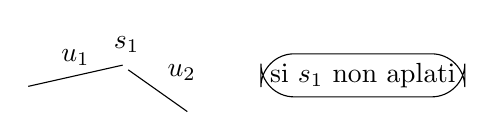
\begin{tikzpicture}
\draw (0,0)--(1.2,.27) node[midway,above] {$u_1$};
\node[above] at (1.25,.3) {$s_1$};
\draw (1.27,.21)--(2.02,-.32) node[midway,above right] {$u_2$};
\node[draw,rounded corners=12pt] at (4.25,.14) {si $s_{1}$ non aplati};
\end{tikzpicture}}

\[\resizebox{\ifdim\width>\linewidth\linewidth\else\width\fi}{!}{$\displaystyle
\begin{aligned}
 &u_0\quad u_1\quad u_2\quad u_3\\
 &u_0\wedge u_1\quad u_1\wedge u_2\quad u_2\wedge u_3\qquad
 \deleted{u_3\wedge u_0=u_3\wedge[\unsure{-}(}\\
 &\hspace{4cm}u_3\wedge u_0=-(u_0+u_1+u_2)\wedge u_0=\\
 &\hspace{5.5cm}\unsure{+|-}u_0\wedge u_1+u_0\wedge u_2
\end{aligned}
$}\]

\figure{\begin{tikzpicture}[x=.011cm,y=-.011cm]
\draw (464,2195)..controls(448,2173)and(397,2150)..(364,2104)--(416,2059);
\draw (431,2042)--(479,1992);
\draw (493,1995)..controls(516,2029)and(537,2060)..(589,2083);
\end{tikzpicture}}
\diagram{\(\begin{array}{cc}x_0&y_0\\x_1&y_1\\x_2&y_2\\x_3&y_3\end{array}\)}
% archive sheet number: 23
